\documentclass{acm_proc_article-sp}
\setlength{\paperheight}{11in}
\setlength{\paperwidth}{8.5in}
\usepackage[pass]{geometry}
\usepackage{subcaption}

\title{Screen-Camera Communications}
\subtitle{}
\author{
    Zhe-Yu Wu, Shao-Chuan Lee, Hsin-Wei Wang, Shao-Tung Chiu, Tsuen-Je Tsai \\
    \affaddr{B02902125, B01902010, B01902048, B01902085, B01902138} \\
    \email{\{B02902125, B01902010, B01902048, B01902085, B01902138\}@csie.ntu.edu.tw}
}

\begin{document}
\maketitle

\begin{abstract}
In this report, we propose a framework that enables concurrent visual communication for both human and devices. Digital watermarking techniques are applied to encode messages into video, while remaining unperceptible to human vision. To make the watermarking invisible, inverse patterns with respect to the original frames' luminance are embedded into consequent frames of the video. At a high frame rate of 60fps, the embedded pattern is not easily seen by human eye. To decode the message, the camera captures the screen at the same frame rate, and patterns are extracted from consecutive frames by cancelling out the original frame. The theoretical bitrate of our approach reaches about 18kbps, not considering redundancy for error correction.
\end{abstract}

\section{Introduction}
Recently, communication systems based on visual content have been developed and applied widely. For example, the QR code have become popular due to its fast detecting, decoding and high storage capacity. In a single QR code, at most 2,953 bytes of data can be stored. Great fault tolerance is also provided in the system, where a QR code can still be decoded with $7\%\sim30\%$ corrupted data.

Unfortunately, such visual patterns are usually device-friendly but not quite consumable by humans. The coded patterns often compromises visual spaces, both temporal and spacial. The trade-off between information delivery and aesthetics has always been bothering visual designers.

The ultimate way to overcome the issue is to encode data such that the original visual content cannot be seen by human eyes. Such a goal is achievable, since human vision is not as sensitive as modern camera-equipped device. Researchers have been working on different encoding methods to minimize human eye perception, and several frameworks have been proposed.

Researches in the field of digital watermarking have also been working on embedding data into static images while reducing visibility of patterns. Developed for tracing copyright infringements and other security purposes, existing approaches are even resistant against image distortion and error.

In this paper, we combine both techniques and propose a novel framework that enables data transmission in video content while not perceptible by humans.

\section{Related Works}
Pervious works on screen-camera communications have been developed. Wang \textit{et al.} proposed \textsc{InFrame++}\cite{wang2015inframe++}, a framework that allows concurrent communication for both users and devices by embedding patterns onto video contents. Their work aims at reducing human perception of data patterns by exploiting characteristics of human vision. In \textsc{InFrame++}, the concept of \textit{temporal complementary frames} is applied: the video frame rate is upsampled by duplicating frames, and patterns are embedded onto the frames such that for each pixel, the average luminance between each 2 frames equals to that of the original frame. The fluctation at $\geq 60$ fps is not perceptible to human eyes due to the low-pass filtering behavior of human vision.

Being well-known in the field of digital watermarking, Cox \textit{et al.}\cite{cox1997secure} proposed a novel watermarking technique on static images which is both perceptually invisible and robust against distortions through a lossy channel. The image is transformed into the frequency domain through 2-dimensional discrete cosine transform, and the watermark is embedded into the frequency components. In their work, eye perception of watermark patterns may be significantly reduced by tuning algorithm parameters.

\section{Structure}
\subsection{Generating Data Patterns}
The carrying data is first transformed into visual patterns. A block of fixed size $c \cdot c$ ($c$ is an even number) pixels is determined as the basic data-carrying unit, where each encodes $n$ bits of the data stream.

To encode $n$ bits, $2^n$ vectors of length $l$ ($l \ll c^2$) are randomly generated from normal distribution. The vectors are then orthogonalized through the Gram-Schmidt process. Since $2^n$ orthogonal vectors are being constructed, the constraint $2^n \leq l$ shall be fulfilled. Each of the $2^n$ vectors represents a $n$-bit symbol.

For each $n$ bits of data, the representing vector is converted into a $c$-by-$c$ matrix in the DCT domain. Since low-frequency components are located in the upper-left region (see Figure \ref{fig:dct8x8}), the vector components are arranged into the upper-left of the matrix, and other components are set to $0$. By performing inverse DCT to the matrix, the resulting pattern block is obtained (an example can be seen in Figure \ref{fig:symbol}). The data pattern frame $D$ is formed by combining all pattern blocks in a frame.

\begin{figure}
    \centering
    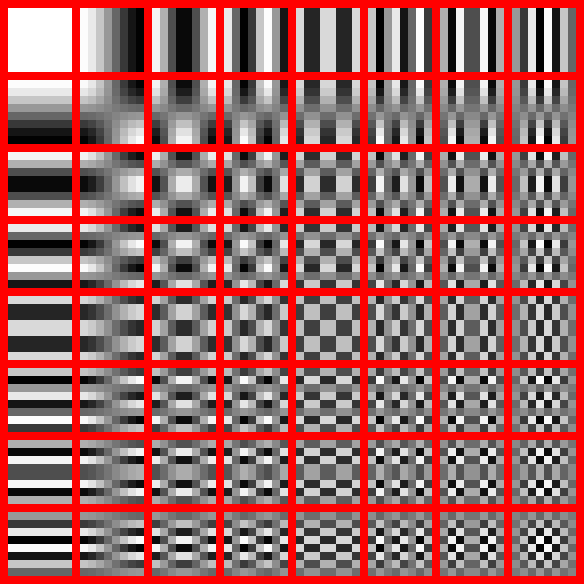
\includegraphics[scale=0.28]{figures/dct8x8}
    \caption{Frequency components in 8x8 DCT.}
    \label{fig:dct8x8}
\end{figure}

\begin{figure}
    \centering
    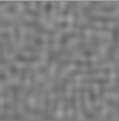
\includegraphics[scale=0.5]{figures/symbol}
    \caption{A 256-bit symbol pattern example on gray background.}
    \label{fig:symbol}
\end{figure}

\subsection{Embedding Pattern into Frames}
The video is processed in the HSV color space, where we only modify the luminance components. Each frame is divided into $\frac{W}{c}\cdot\frac{H}{c}$ blocks for embedding patterns, where $W$ and $H$ denote the width and height of the video, respectively, assuming both $W$ and $H$ are multiples of $c$. Since we are to embed the patterns by increasing/reducing the luminance level, we first scale the luminance of each pixel as follows:
\begin{equation}
V' = 0.8V + 25.6
\end{equation}
where $V$ and $V'$ represent the luminance level matrix of the original and scaled frames, respectively.

Let $f$ denote the original frame rate of the video. During embedding, each frame is duplicated, resulting in doubled frame rate $2f$. For each pair of duplicating frames, we add the data pattern $D$ onto the first frame, and subtract $D$ from the second. A scaling factor $\alpha$ may be added to adjust signal strength. The two frames $V'+\alpha D$ and $V'-\alpha D$ forms temporal complementary frames, and the data pattern will thus become hardly human-perceptible.

An additional border is added to the video, and QR code-like locators are placed in the corners, as shown in Figure \ref{fig:locator}. In real-world applications, physical locators may be placed around the screen to avoid compromising space.

\begin{figure}
    \centering
    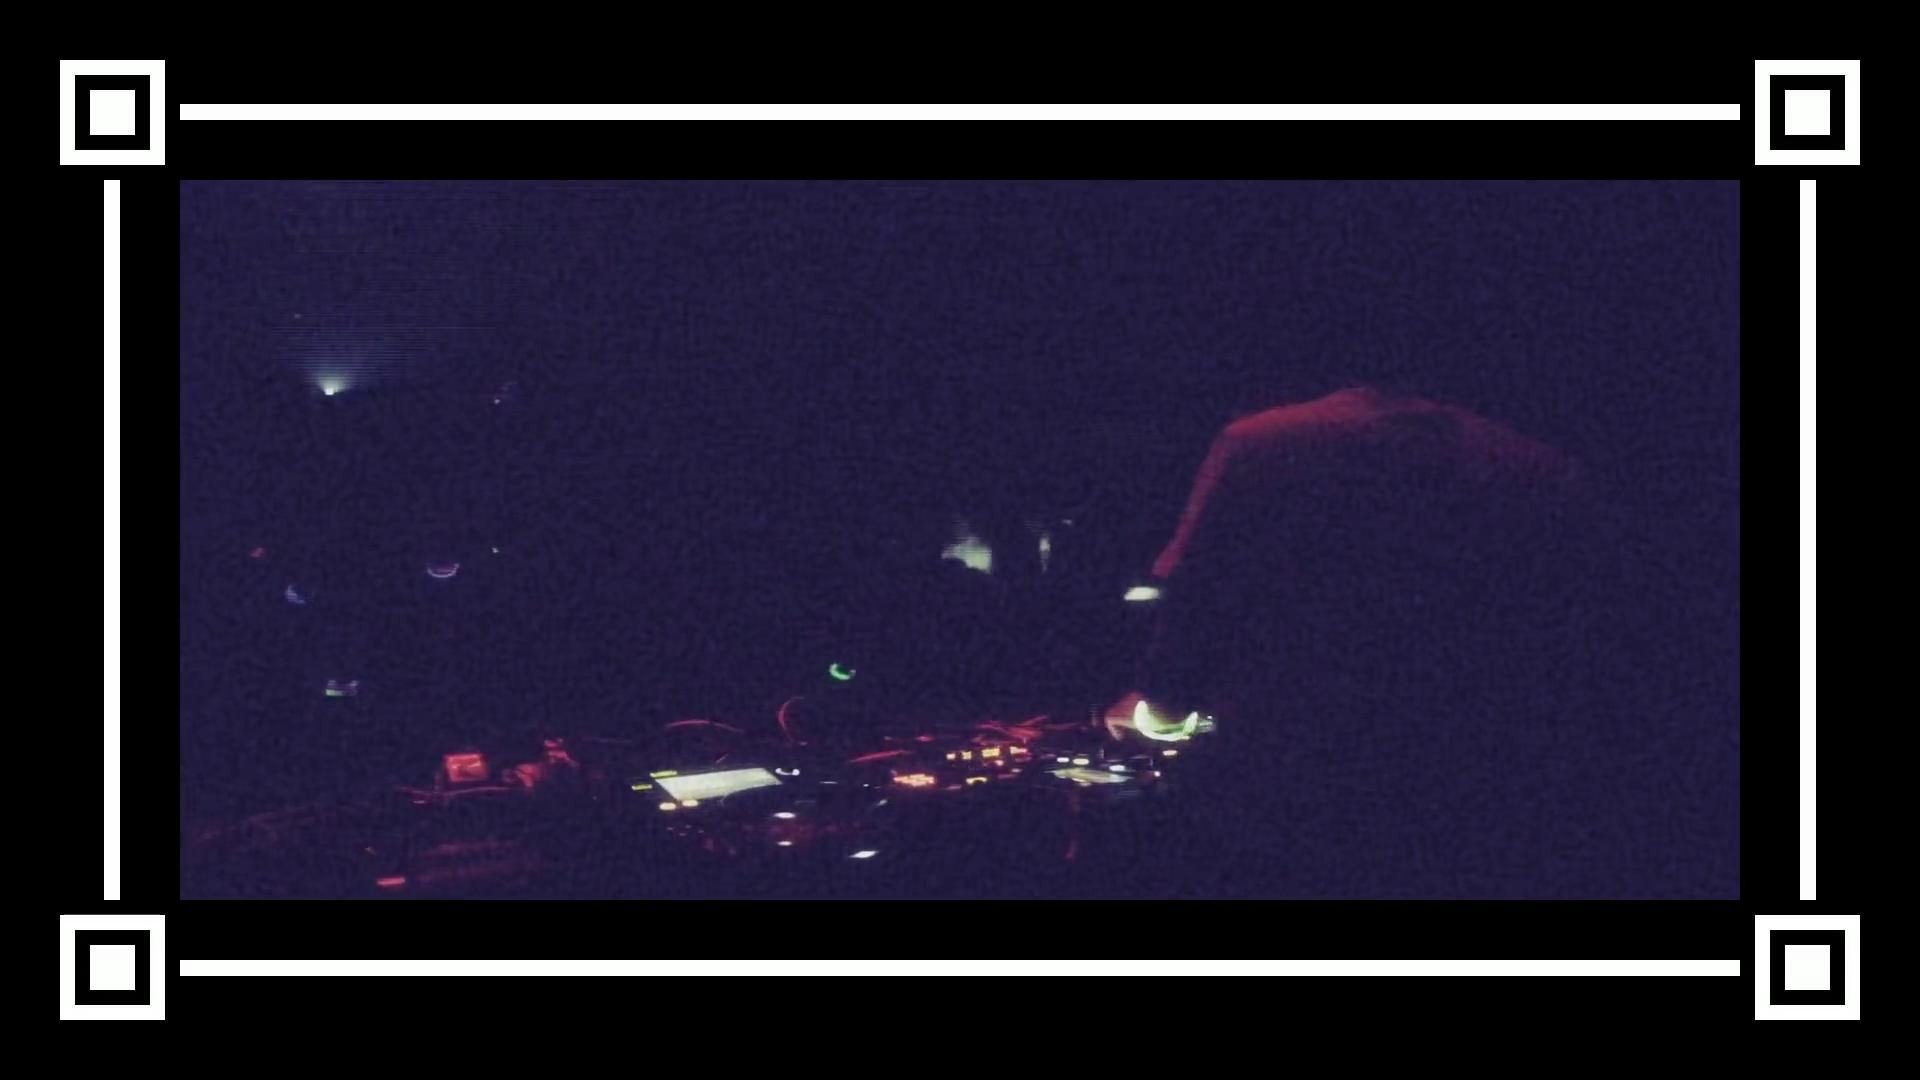
\includegraphics[width=\linewidth]{figures/locator}
    \caption{An encoded video frame with locators.}
    \label{fig:locator}
\end{figure}

\subsection{Decoding}
In order to correctly divide the frame into blocks, video captured by cameras are first located and calibrated. Keystone correction is applied to the captured frames according to locators, and the frames are cropped to contain only the encoded video.

For each pair of temporal complementary frames constructed during encoding, the first frame $V'+\alpha D$ is subtracted by the second frame $V'-\alpha D$, extracting the encoded pattern frame $D$. The pattern frame is further divided into blocks, and the correct symbol is detected by calculating the standard inner product between the decoded pattern and all possible symbol patterns, and find the symbol that produces the largest outcome.

\section{Experimental Setup and Results}
In our experiment, the Eizo EV2336W monitor is used for 1920x1080@60fps video playback, and Canon EOS 70D is used for screen capturing at 1280x720@60fps. The captured frames are offline processed in a separate computer. Block size $c = 120$ pixels is chosen, each encoding a byte with $2^8 = 256$ symbols. A border of 360 pixels is added, resulting in 1560x720 video frames containing 78 blocks.

Two video samples are used for performance evaluation: (1) ``anime'' with large color blocks and bold drawing lines, and (2) ``concert'' consisting of complex details and fast-alternating scenes.

First we evaluate the bit error rate (BER) with different number of total symbols, signal strength factor $\alpha$ fixed at $0.6$. As shown in Figure \ref{fig:ber-symbols}, there is a positive correlation between the number of symbols and the BER. Although BER is reaching $25\%$ when each block represents a byte, data may still be recovered with error correction techniques, with redundancy added to the original data stream. In our implementation, we adopted the Reed-Solomon error correction\cite{reed1960polynomial}, in which the redundancy factor $t$ can be tuned to correct at most $\lfloor\frac{t}{2}\rfloor$ symbols by adding $t$ additional symbols.

\begin{figure}[t]
    \centering
    
\end{figure}

We also evaluated error rates at different signal strength factors, since we want the factor as small as possible to avoid human perception of encoded patterns. Results are shown in Figure \ref{fig:ber-alpha}, where negative correlation is found between $\alpha$ and BER. At $\alpha = 0.2$, the BER of both video samples are reaching $0.5$, which is nearly impossible to decode. Setting $\alpha \geq 0.4$ seems to be applicable with error-correcting codes.

\begin{figure*}
    \centering
    \begin{subfigure}[b]{0.48\linewidth}
        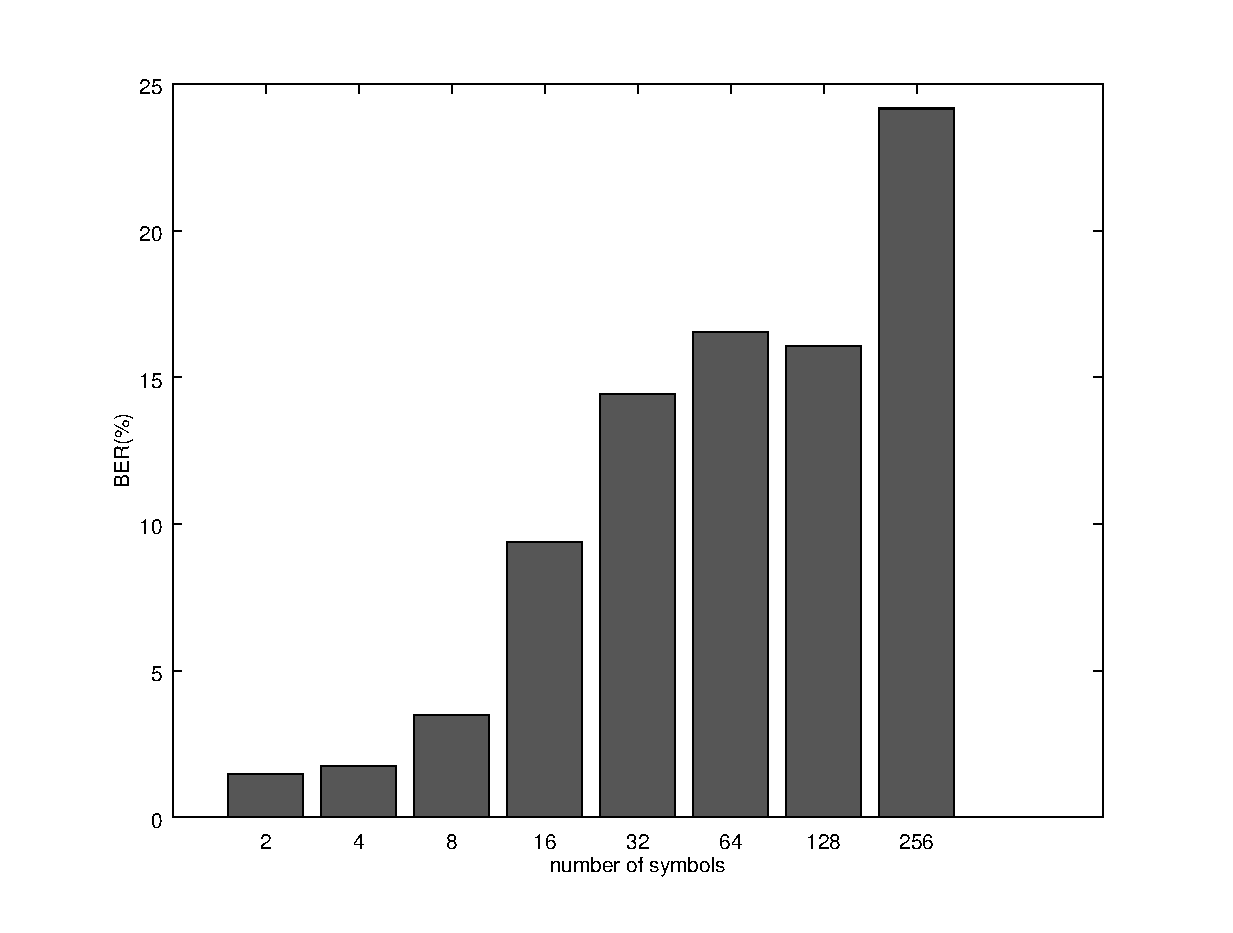
\includegraphics[width=\linewidth]{figures/ber-symbols}
        \caption{BER at different numbers of symbols per block.}
        \label{fig:ber-symbols}
    \end{subfigure}
    \begin{subfigure}[b]{0.48\linewidth}
        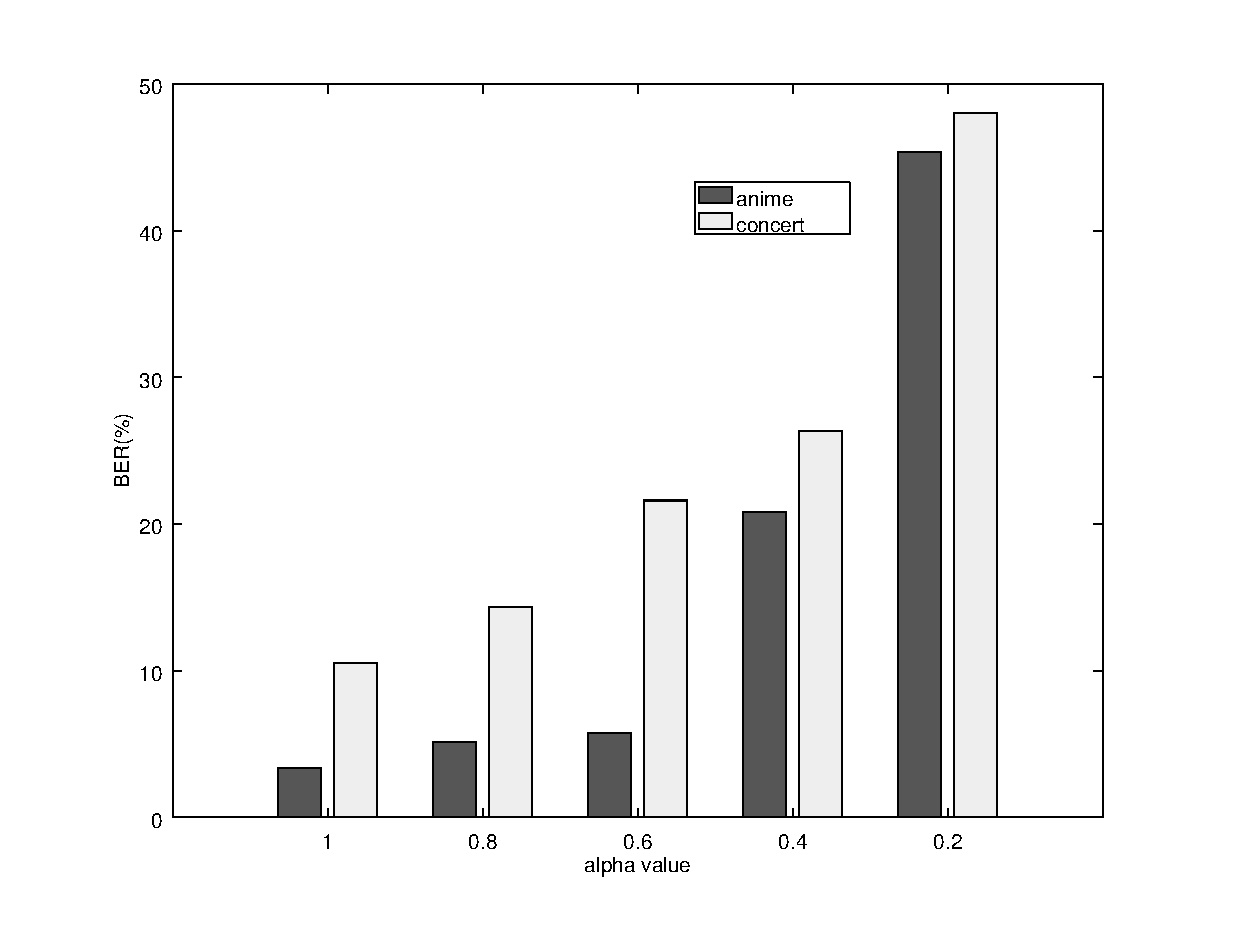
\includegraphics[width=\linewidth]{figures/ber-alpha}
        \caption{BER at different strength factor $\alpha$.}
        \label{fig:ber-alpha}
    \end{subfigure}
    \caption{Evaluated results.}
\end{figure*}

The theoretical bitrate in our settings is $n \cdot \frac{WH}{c^2} \cdot f = 18$kbps; however, in practice the bitrate varies by channel quality, signal strength and redundancy factors.

\section{Conclusion}
In this report, we proposed a novel framework for encoding data into video content while not perceptible by human vision. By adopting digital watermarking as well as exploiting human vision characteristics, we achieved invisible data transfer at 60fps, compared to previous works that requires a 120fps display. By resolving the problem of temporal/spacial consumption of current approaches like the QR code, additional information may be delivered with video in a much more comfortable way.

However, our current method requires the video frame to be located, since data are encoded block-by-block. We have come up with a new method by using the 2D-FFT (two-dimensional fast fourier transform) technique for encoding and decoding. The concept of new method is similar to the current work, but the frequency domain of 2D-FFT contains phase information, which enables the frame to be decoded with imprecise position. The frames are decoded by detecting the magnitudes in the frequency domain, and incorrect phases influenced by the position of the frame are ignored. Locating is unnecessary under such design, and aesthetics is guaranteed.

\bibliographystyle{acm}
\bibliography{report}

\end{document}